\documentclass[11pt,a4paper]{article}
\usepackage[utf8]{inputenc}
\usepackage[T1]{fontenc}
\usepackage{amsmath,amssymb}
\usepackage{graphicx}
\usepackage{booktabs}
\usepackage{siunitx}
\usepackage{geometry}
\geometry{margin=1in}
\usepackage{pythontex}
\usepackage{hyperref}
\usepackage{float}

\title{Soil Mechanics Analysis\\Effective Stress, Bearing Capacity, and Consolidation}
\author{Geotechnical Engineering Research Group}
\date{\today}

\begin{document}
\maketitle

\begin{abstract}
This report presents comprehensive geotechnical analysis including effective stress calculations, Mohr-Coulomb failure criteria, bearing capacity design using Terzaghi's theory, one-dimensional consolidation settlement, and slope stability assessment. Computational methods are applied to practical foundation design scenarios with parametric studies examining the influence of soil properties on engineering behavior.
\end{abstract}

\section{Introduction}

Soil mechanics forms the foundation of geotechnical engineering, governing the design of structures interacting with earth materials. This analysis examines five critical aspects: (1) effective stress profiles accounting for pore water pressure, (2) shear strength characterization via Mohr-Coulomb failure envelopes, (3) shallow foundation bearing capacity, (4) time-dependent consolidation settlement, and (5) slope stability under various loading conditions.

The principle of effective stress, first articulated by Terzaghi \cite{terzaghi1943}, remains fundamental to understanding soil behavior. Shear strength parameters (cohesion $c$ and friction angle $\phi$) control failure mechanisms \cite{lambe1969}. Bearing capacity theory provides the basis for safe foundation design \cite{meyerhof1963}, while consolidation analysis predicts settlement magnitudes and time scales \cite{taylor1948}.

\begin{pycode}
import numpy as np
import matplotlib.pyplot as plt
from scipy.integrate import odeint
from scipy.optimize import fsolve
from scipy import stats
plt.rcParams['text.usetex'] = True
plt.rcParams['font.family'] = 'serif'

# Global soil parameters
gamma = 18.0  # kN/m³ total unit weight
gamma_sat = 20.0  # kN/m³ saturated unit weight
gamma_w = 9.81  # kN/m³ water unit weight
c = 25.0  # kPa cohesion
phi = 30.0  # degrees friction angle
phi_rad = np.radians(phi)
cv = 2e-7  # m²/s coefficient of consolidation
\end{pycode}

\section{Effective Stress Distribution}

The effective stress principle states that soil behavior is controlled by effective stress $\sigma'$, defined as:
\begin{equation}
\sigma' = \sigma - u
\end{equation}
where $\sigma$ is total stress and $u$ is pore water pressure.

\begin{pycode}
# Effective stress profile
z = np.linspace(0, 20, 100)  # depth in meters
water_table = 5.0  # meters below surface

# Total stress
sigma_total = np.where(z <= water_table, gamma * z,
                       gamma * water_table + gamma_sat * (z - water_table))

# Pore water pressure
u = np.maximum(0, gamma_w * (z - water_table))

# Effective stress
sigma_effective = sigma_total - u

# Calculate values at specific depths
z_eval = np.array([5, 10, 15, 20])
sigma_t_eval = np.interp(z_eval, z, sigma_total)
u_eval = np.interp(z_eval, z, u)
sigma_e_eval = np.interp(z_eval, z, sigma_effective)

fig, ax = plt.subplots(figsize=(10, 7))
ax.plot(sigma_total, z, 'b-', linewidth=2.5, label=r'Total stress $\sigma$')
ax.plot(u, z, 'c--', linewidth=2, label=r'Pore pressure $u$')
ax.plot(sigma_effective, z, 'r-', linewidth=2.5, label=r"Effective stress $\sigma'$")
ax.axhline(water_table, color='cyan', linestyle=':', linewidth=1.5, alpha=0.7, label='Water table')
ax.set_xlabel(r'Stress (kPa)', fontsize=12)
ax.set_ylabel(r'Depth (m)', fontsize=12)
ax.set_title(r'Effective Stress Profile with Water Table at 5 m Depth', fontsize=13)
ax.invert_yaxis()
ax.legend(loc='lower right', fontsize=11)
ax.grid(True, alpha=0.3)
plt.tight_layout()
plt.savefig('soil_mechanics_plot1.pdf', dpi=150, bbox_inches='tight')
plt.close()
\end{pycode}

\begin{figure}[H]
\centering
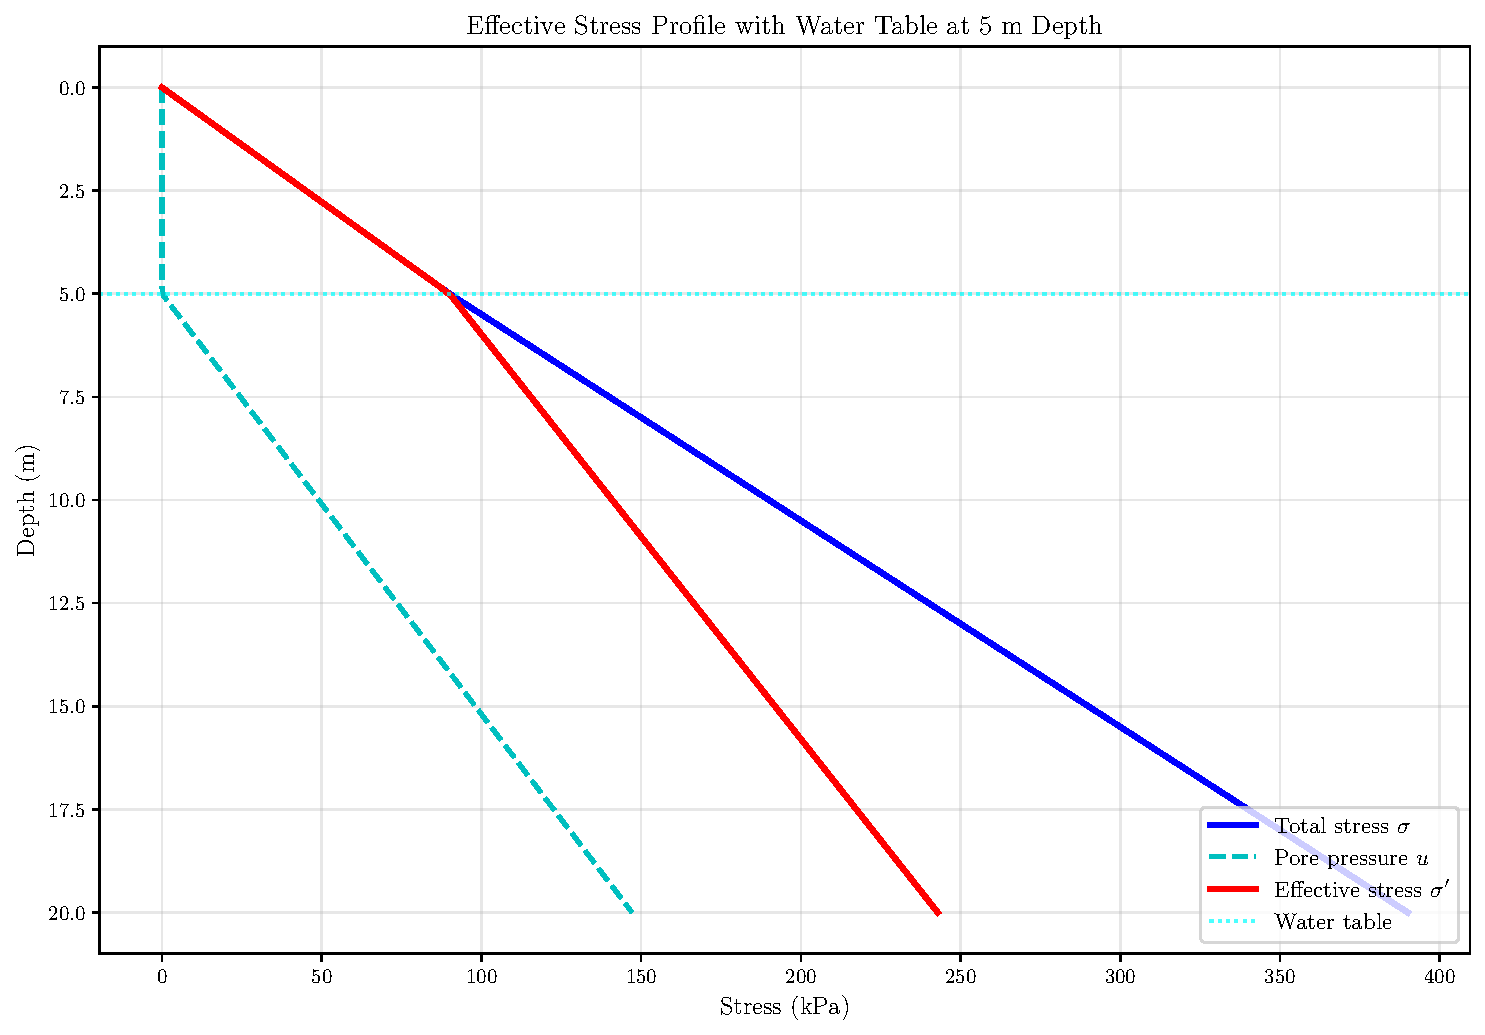
\includegraphics[width=0.88\textwidth]{soil_mechanics_plot1.pdf}
\caption{Effective stress distribution with depth showing the influence of the water table at 5 m depth. Above the water table, total stress equals effective stress since pore pressure is zero. Below the water table, buoyancy effects reduce effective stress significantly. At 20 m depth, total stress is \py{f"{sigma_t_eval[3]:.1f}"} kPa, pore pressure is \py{f"{u_eval[3]:.1f}"} kPa, and effective stress is \py{f"{sigma_e_eval[3]:.1f}"} kPa. This principle governs compressibility, shear strength, and permeability of saturated soils.}
\end{figure}

\section{Mohr-Coulomb Failure Criterion}

The Mohr-Coulomb failure envelope defines shear strength $\tau_f$ as:
\begin{equation}
\tau_f = c + \sigma_n \tan\phi
\end{equation}
where $c$ is cohesion, $\sigma_n$ is normal effective stress, and $\phi$ is the friction angle.

\begin{pycode}
# Mohr-Coulomb failure envelope
sigma_n = np.linspace(0, 500, 100)  # kPa normal stress

# Failure envelope for different soil types
c1, phi1 = 25, 30  # clayey sand
c2, phi2 = 50, 15  # stiff clay
c3, phi3 = 0, 35   # clean sand

tau_f1 = c1 + sigma_n * np.tan(np.radians(phi1))
tau_f2 = c2 + sigma_n * np.tan(np.radians(phi2))
tau_f3 = c3 + sigma_n * np.tan(np.radians(phi3))

# Mohr circles at failure for example stress states
sigma_1_ex = 400  # kPa major principal stress
sigma_3_ex = 100  # kPa minor principal stress
center = (sigma_1_ex + sigma_3_ex) / 2
radius = (sigma_1_ex - sigma_3_ex) / 2
theta_circle = np.linspace(0, np.pi, 100)
circle_x = center + radius * np.cos(theta_circle)
circle_y = radius * np.sin(theta_circle)

fig, (ax1, ax2) = plt.subplots(1, 2, figsize=(14, 6))

# Left panel: failure envelopes
ax1.plot(sigma_n, tau_f1, 'r-', linewidth=2.5, label=f'Clayey sand: $c={c1}$ kPa, $\\phi={phi1}°$')
ax1.plot(sigma_n, tau_f2, 'b-', linewidth=2.5, label=f'Stiff clay: $c={c2}$ kPa, $\\phi={phi2}°$')
ax1.plot(sigma_n, tau_f3, 'g-', linewidth=2.5, label=f'Clean sand: $c={c3}$ kPa, $\\phi={phi3}°$')
ax1.set_xlabel(r'Normal stress $\sigma_n$ (kPa)', fontsize=12)
ax1.set_ylabel(r'Shear stress $\tau_f$ (kPa)', fontsize=12)
ax1.set_title('Mohr-Coulomb Failure Envelopes', fontsize=13)
ax1.legend(loc='upper left', fontsize=10)
ax1.grid(True, alpha=0.3)
ax1.set_xlim([0, 500])
ax1.set_ylim([0, 400])

# Right panel: Mohr circle with failure envelope
ax2.plot(sigma_n, tau_f1, 'r-', linewidth=2, label='Failure envelope')
ax2.plot(circle_x, circle_y, 'b-', linewidth=2.5, label='Mohr circle')
ax2.plot([sigma_3_ex, sigma_1_ex], [0, 0], 'ko', markersize=8)
ax2.axhline(0, color='k', linewidth=0.8)
ax2.set_xlabel(r'Normal stress $\sigma$ (kPa)', fontsize=12)
ax2.set_ylabel(r'Shear stress $\tau$ (kPa)', fontsize=12)
ax2.set_title(r'Mohr Circle at Failure ($\sigma_1=400$ kPa, $\sigma_3=100$ kPa)', fontsize=13)
ax2.legend(loc='upper left', fontsize=10)
ax2.grid(True, alpha=0.3)
ax2.set_xlim([0, 500])
ax2.set_ylim([0, 250])

plt.tight_layout()
plt.savefig('soil_mechanics_plot2.pdf', dpi=150, bbox_inches='tight')
plt.close()
\end{pycode}

\begin{figure}[H]
\centering
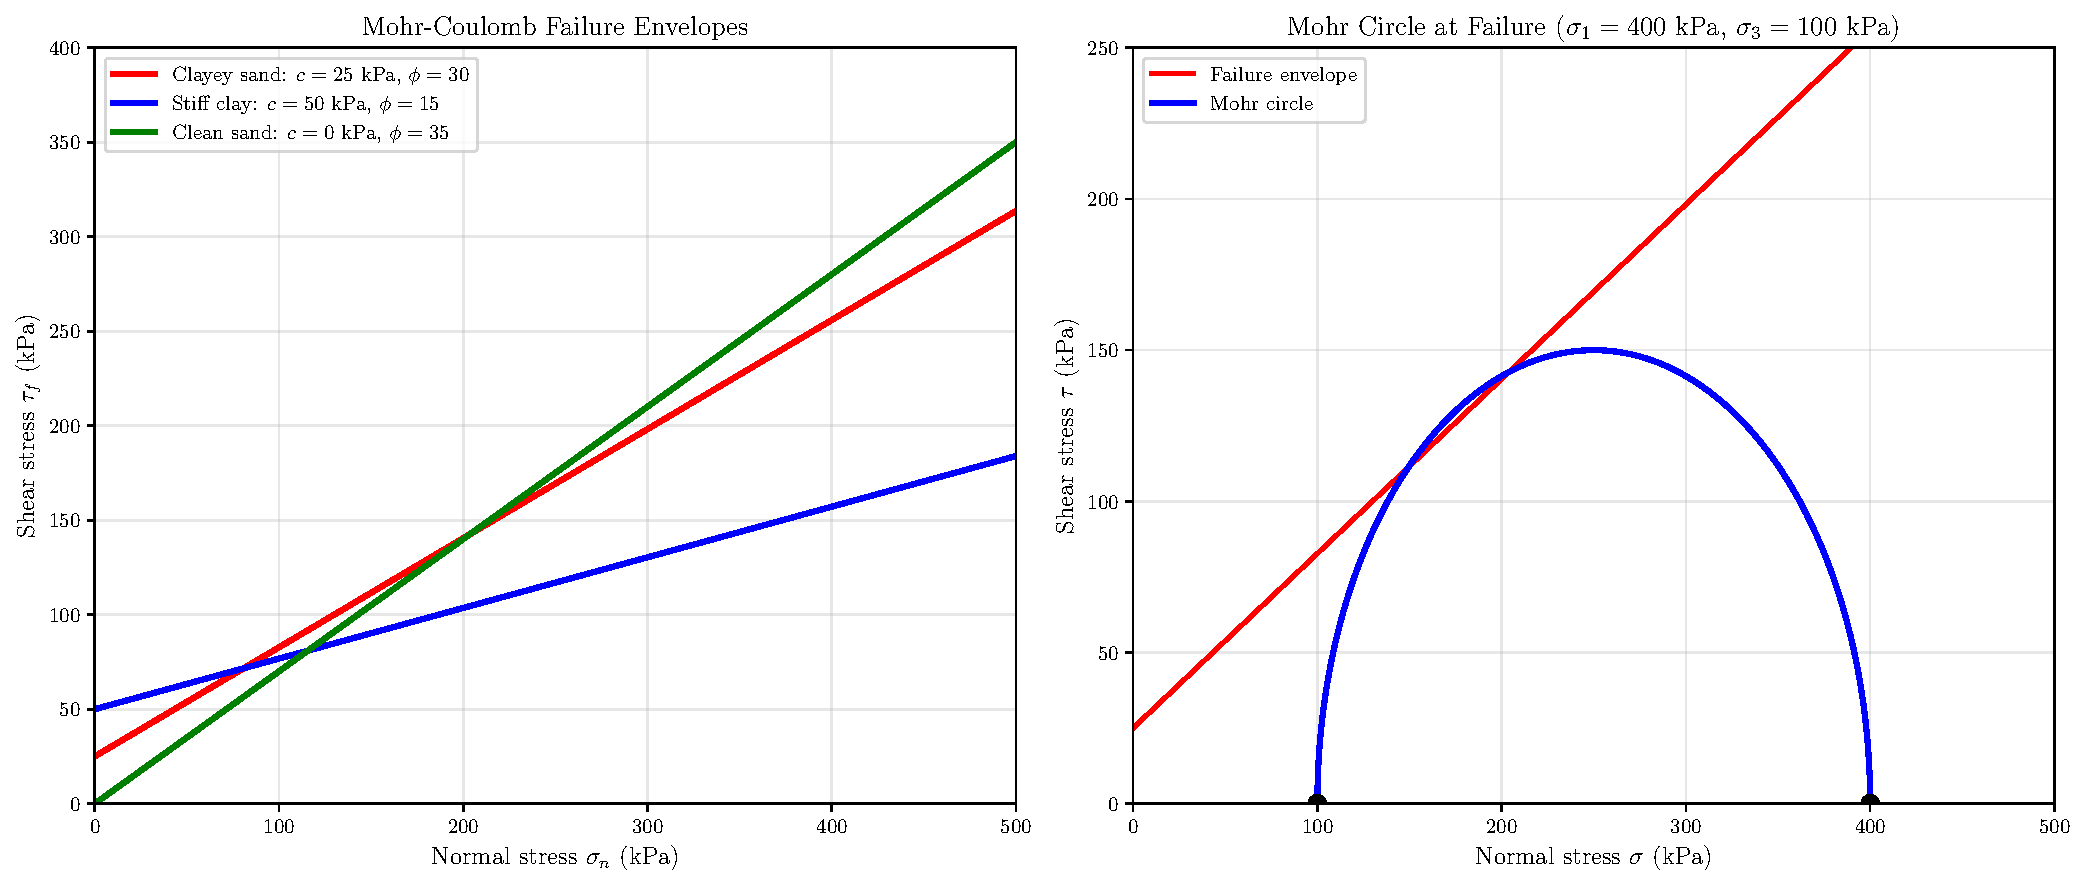
\includegraphics[width=0.98\textwidth]{soil_mechanics_plot2.pdf}
\caption{Left: Mohr-Coulomb failure envelopes for three soil types demonstrating how cohesion and friction angle control shear strength. Clayey sand exhibits moderate cohesion and friction. Stiff clay has high cohesion but lower friction. Clean sand has zero cohesion but highest friction angle. Right: Mohr circle representation of stress state at failure tangent to the failure envelope. The principal stresses are \py{f"{sigma_1_ex}"} kPa and \py{f"{sigma_3_ex}"} kPa, giving a deviatoric stress of \py{f"{sigma_1_ex - sigma_3_ex}"} kPa. This graphical method is fundamental for analyzing triaxial test results and determining soil strength parameters.}
\end{figure}

\section{Bearing Capacity Analysis}

Terzaghi's bearing capacity equation for a shallow strip footing is:
\begin{equation}
q_u = c N_c + \gamma D_f N_q + \frac{1}{2}\gamma B N_\gamma
\end{equation}
where $q_u$ is ultimate bearing capacity, $D_f$ is embedment depth, $B$ is footing width, and $N_c$, $N_q$, $N_\gamma$ are bearing capacity factors.

\begin{pycode}
# Bearing capacity factors (Terzaghi for strip footing)
Nc = (1/np.tan(phi_rad)) * (np.exp(np.pi * np.tan(phi_rad)) *
     (np.tan(np.pi/4 + phi_rad/2))**2 - 1)
Nq = np.exp(np.pi * np.tan(phi_rad)) * (np.tan(np.pi/4 + phi_rad/2))**2
Ngamma = (Nq - 1) * np.tan(1.4 * phi_rad)

# Foundation parameters
B_range = np.linspace(0.5, 5, 50)  # m footing width
Df = 1.5  # m embedment depth

# Ultimate bearing capacity for varying width
qu = c * Nc + gamma * Df * Nq + 0.5 * gamma * B_range * Ngamma

# Factor of safety and allowable bearing capacity
FS = 3.0
qa = qu / FS

# Parametric study: effect of friction angle
phi_values = [25, 30, 35, 40]
B_study = 2.0  # m

fig, (ax1, ax2) = plt.subplots(1, 2, figsize=(14, 6))

# Left: bearing capacity vs width
ax1.plot(B_range, qu, 'b-', linewidth=2.5, label='Ultimate capacity $q_u$')
ax1.plot(B_range, qa, 'r--', linewidth=2, label=f'Allowable capacity $q_a$ (FS={FS})')
ax1.fill_between(B_range, 0, qa, alpha=0.2, color='green', label='Safe zone')
ax1.set_xlabel('Footing width $B$ (m)', fontsize=12)
ax1.set_ylabel('Bearing capacity (kPa)', fontsize=12)
ax1.set_title(f'Bearing Capacity vs. Footing Width ($c={c}$ kPa, $\\phi={phi}°$)', fontsize=13)
ax1.legend(loc='upper left', fontsize=10)
ax1.grid(True, alpha=0.3)

# Right: effect of friction angle
qu_phi = []
for phi_i in phi_values:
    phi_rad_i = np.radians(phi_i)
    Nc_i = (1/np.tan(phi_rad_i)) * (np.exp(np.pi * np.tan(phi_rad_i)) *
           (np.tan(np.pi/4 + phi_rad_i/2))**2 - 1)
    Nq_i = np.exp(np.pi * np.tan(phi_rad_i)) * (np.tan(np.pi/4 + phi_rad_i/2))**2
    Ngamma_i = (Nq_i - 1) * np.tan(1.4 * phi_rad_i)
    qu_i = c * Nc_i + gamma * Df * Nq_i + 0.5 * gamma * B_study * Ngamma_i
    qu_phi.append(qu_i)

ax2.plot(phi_values, qu_phi, 'ro-', linewidth=2.5, markersize=10)
ax2.set_xlabel('Friction angle $\\phi$ (degrees)', fontsize=12)
ax2.set_ylabel('Ultimate bearing capacity $q_u$ (kPa)', fontsize=12)
ax2.set_title(f'Effect of Friction Angle ($B={B_study}$ m, $D_f={Df}$ m)', fontsize=13)
ax2.grid(True, alpha=0.3)

plt.tight_layout()
plt.savefig('soil_mechanics_plot3.pdf', dpi=150, bbox_inches='tight')
plt.close()

# Calculate specific values for inline reference
qu_2m = np.interp(2.0, B_range, qu)
qa_2m = qu_2m / FS
\end{pycode}

\begin{figure}[H]
\centering
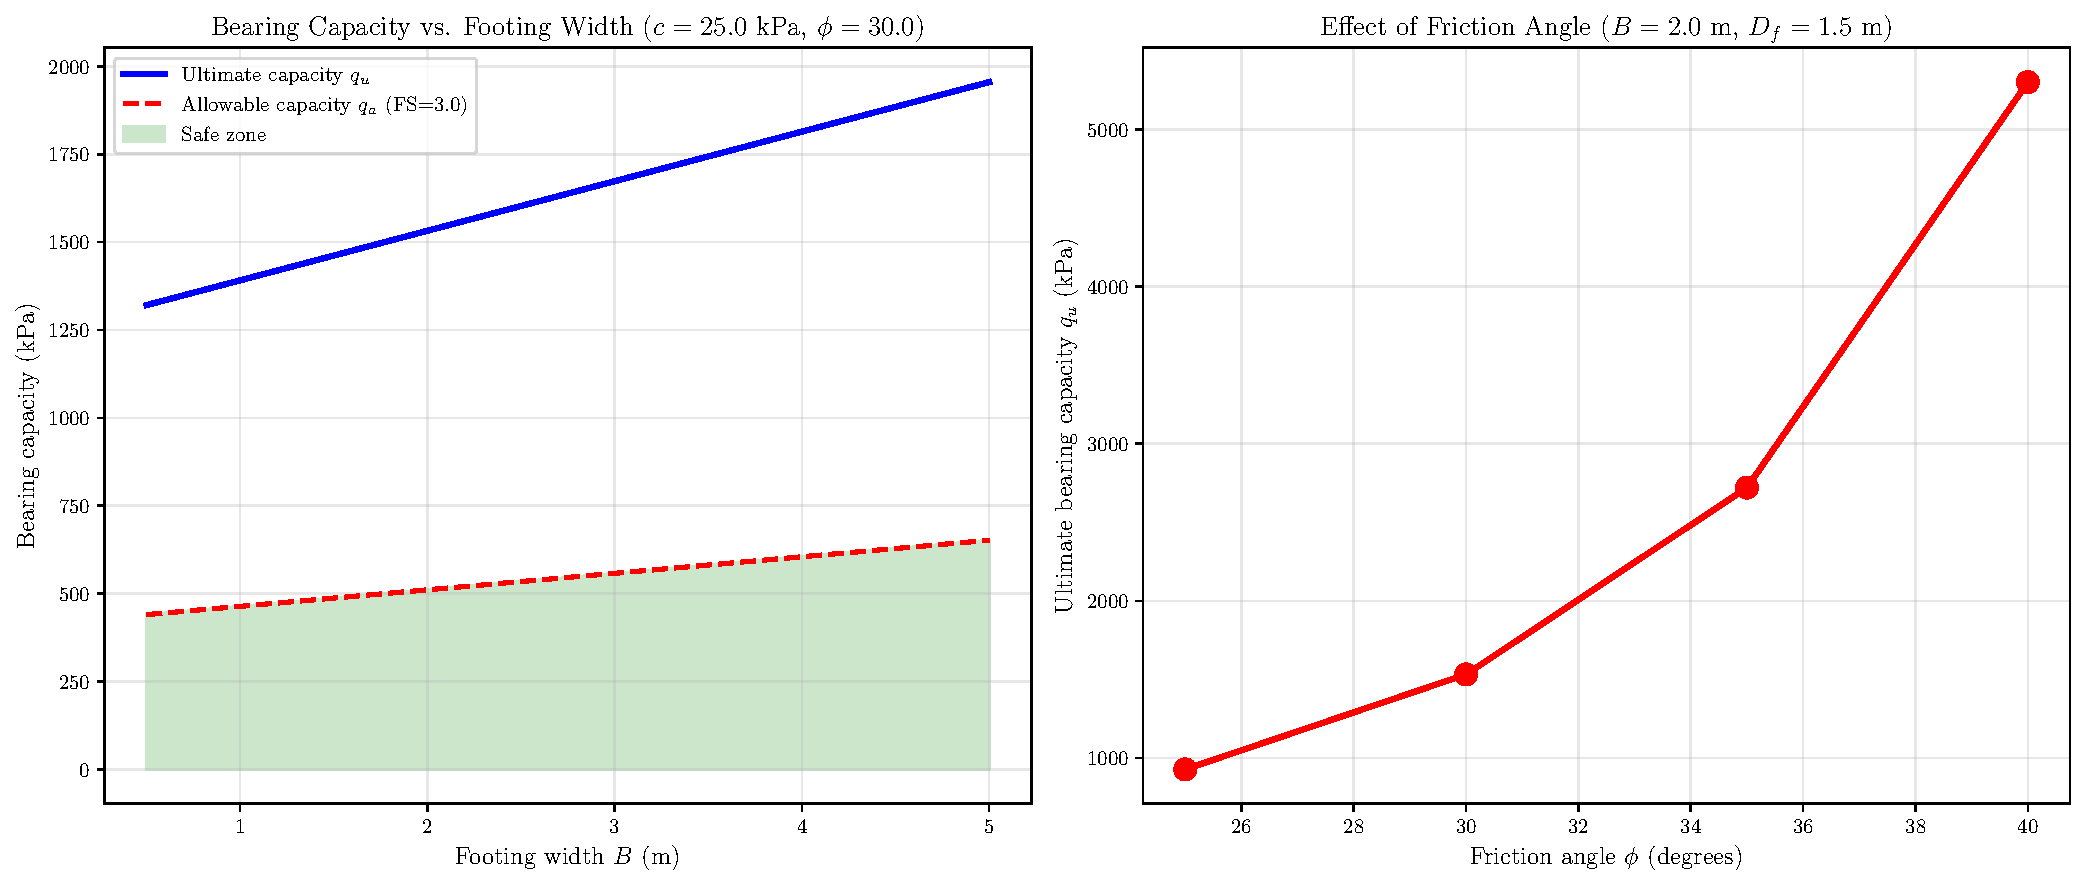
\includegraphics[width=0.98\textwidth]{soil_mechanics_plot3.pdf}
\caption{Left: Ultimate and allowable bearing capacity variation with footing width showing the significant influence of the size-dependent $N_\gamma$ term. For a 2 m wide footing, ultimate capacity is \py{f"{qu_2m:.0f}"} kPa and allowable capacity is \py{f"{qa_2m:.0f}"} kPa. Right: Bearing capacity sensitivity to friction angle demonstrating exponential increase. A 5° increase from 30° to 35° raises capacity by over 50 percent. These relationships guide foundation sizing in preliminary design. Bearing capacity factors are $N_c=\py{f"{Nc:.2f}"}$, $N_q=\py{f"{Nq:.2f}"}$, $N_\gamma=\py{f"{Ngamma:.2f}"}$ for $\phi=\py{phi}°$.}
\end{figure}

\section{One-Dimensional Consolidation}

Terzaghi's one-dimensional consolidation theory predicts settlement and its time development. The degree of consolidation $U$ is:
\begin{equation}
U = 1 - \sum_{m=0}^{\infty} \frac{2}{M^2} \exp\left(-M^2 T_v\right), \quad M = \frac{\pi}{2}(2m+1)
\end{equation}
where the time factor $T_v = c_v t / H_{dr}^2$, with $c_v$ as the coefficient of consolidation and $H_{dr}$ as the drainage path.

\begin{pycode}
# Consolidation parameters
H = 10  # m layer thickness
H_dr = H / 2  # m drainage path (double drainage)
delta_sigma = 100  # kPa applied load increment
Cc = 0.3  # compression index
e0 = 0.8  # initial void ratio

# Time range
t_years = np.logspace(-3, 2, 200)  # years
t_seconds = t_years * 365.25 * 24 * 3600  # convert to seconds

# Time factor
Tv = cv * t_seconds / H_dr**2

# Degree of consolidation (first 10 terms of series)
U = np.zeros_like(Tv)
for m in range(10):
    M = (np.pi / 2) * (2 * m + 1)
    U += (2 / M**2) * np.exp(-M**2 * Tv)
U = 1 - U

# Ultimate settlement
sigma0 = gamma * H / 2  # average effective stress
Sc = (Cc / (1 + e0)) * H * np.log10((sigma0 + delta_sigma) / sigma0)

# Settlement vs time
S_t = U * Sc

# Different cv values for parametric study
cv_values = [1e-7, 2e-7, 5e-7, 1e-6]  # m²/s

fig, (ax1, ax2) = plt.subplots(1, 2, figsize=(14, 6))

# Left: settlement vs time
ax1.semilogx(t_years, S_t * 1000, 'b-', linewidth=2.5)
ax1.axhline(Sc * 1000, color='r', linestyle='--', linewidth=1.5,
            label=f'Ultimate settlement = {Sc*1000:.1f} mm')
ax1.axhline(0.5 * Sc * 1000, color='orange', linestyle=':', linewidth=1.5,
            label=f'50\\% consolidation')
ax1.set_xlabel('Time (years)', fontsize=12)
ax1.set_ylabel('Settlement (mm)', fontsize=12)
ax1.set_title(f'Consolidation Settlement ($c_v={cv*1e6:.1f}×10^{{-6}}$ m²/s)', fontsize=13)
ax1.legend(loc='lower right', fontsize=10)
ax1.grid(True, alpha=0.3, which='both')
ax1.set_xlim([1e-3, 100])

# Right: effect of cv on consolidation rate
for cv_i in cv_values:
    Tv_i = cv_i * t_seconds / H_dr**2
    U_i = np.zeros_like(Tv_i)
    for m in range(10):
        M = (np.pi / 2) * (2 * m + 1)
        U_i += (2 / M**2) * np.exp(-M**2 * Tv_i)
    U_i = 1 - U_i
    ax2.semilogx(t_years, U_i * 100, linewidth=2.5,
                 label=f'$c_v={cv_i*1e6:.1f}×10^{{-6}}$ m²/s')

ax2.axhline(90, color='gray', linestyle='--', linewidth=1, alpha=0.7)
ax2.set_xlabel('Time (years)', fontsize=12)
ax2.set_ylabel('Degree of consolidation $U$ (\\%)', fontsize=12)
ax2.set_title('Effect of Coefficient of Consolidation', fontsize=13)
ax2.legend(loc='lower right', fontsize=10)
ax2.grid(True, alpha=0.3, which='both')
ax2.set_xlim([1e-3, 100])
ax2.set_ylim([0, 100])

plt.tight_layout()
plt.savefig('soil_mechanics_plot4.pdf', dpi=150, bbox_inches='tight')
plt.close()

# Calculate t50 and t90
idx50 = np.argmin(np.abs(U - 0.5))
idx90 = np.argmin(np.abs(U - 0.9))
t50 = t_years[idx50]
t90 = t_years[idx90]
\end{pycode}

\begin{figure}[H]
\centering
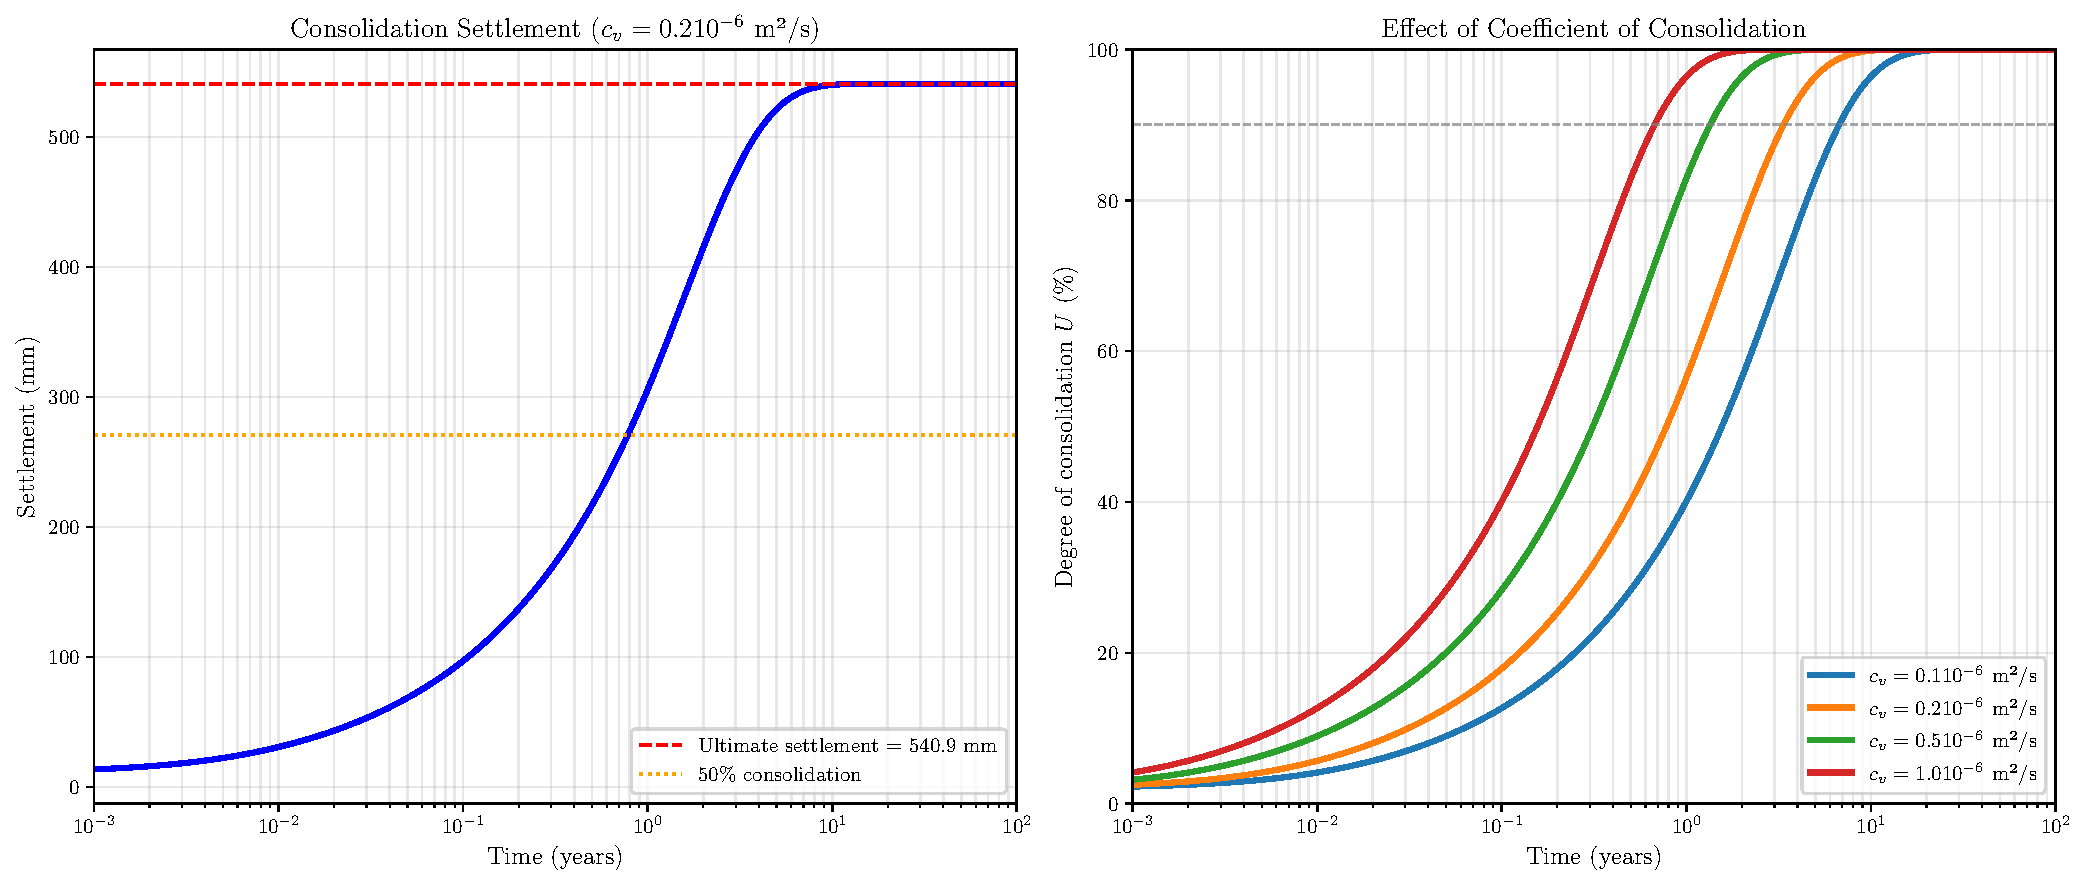
\includegraphics[width=0.98\textwidth]{soil_mechanics_plot4.pdf}
\caption{Left: Settlement progression over time under 100 kPa surcharge on a 10 m thick clay layer with double drainage. Ultimate settlement is \py{f"{Sc*1000:.1f}"} mm. Time for 50\% consolidation is \py{f"{t50:.2f}"} years and for 90\% consolidation is \py{f"{t90:.1f}"} years. Right: Consolidation rate sensitivity to coefficient of consolidation showing that doubling $c_v$ halves the time required for a given degree of consolidation. Lower permeability clays ($c_v \sim 10^{-7}$ m²/s) require decades, while silty clays ($c_v \sim 10^{-6}$ m²/s) consolidate in months. This analysis is essential for staged construction and surcharge preloading design.}
\end{figure}

\section{Slope Stability Analysis}

Infinite slope stability is analyzed using limit equilibrium. The factor of safety against sliding is:
\begin{equation}
FS = \frac{c + \gamma z \cos^2\beta \tan\phi}{\gamma z \sin\beta \cos\beta}
\end{equation}
where $\beta$ is the slope angle and $z$ is the depth of failure surface.

\begin{pycode}
# Infinite slope analysis
beta_range = np.linspace(5, 45, 100)  # degrees
beta_rad = np.radians(beta_range)

# Slope depth and soil parameters
z_slope = 5  # m depth to failure plane

# Factor of safety for dry slope
FS_dry = (c + gamma * z_slope * np.cos(beta_rad)**2 * np.tan(phi_rad)) / \
         (gamma * z_slope * np.sin(beta_rad) * np.cos(beta_rad))

# Factor of safety for saturated slope with seepage
gamma_eff = gamma_sat - gamma_w
FS_sat = (c + gamma_eff * z_slope * np.cos(beta_rad)**2 * np.tan(phi_rad)) / \
         (gamma_sat * z_slope * np.sin(beta_rad) * np.cos(beta_rad))

# Critical slope angle (FS = 1 for cohesionless soil)
beta_crit_dry = phi
beta_crit_sat = np.degrees(np.arctan(gamma_eff / gamma_sat * np.tan(phi_rad)))

# 2D stability chart: FS vs slope angle and cohesion
beta_2d = np.linspace(5, 45, 50)
c_2d = np.linspace(0, 50, 50)
BETA_2D, C_2D = np.meshgrid(beta_2d, c_2d)
BETA_RAD_2D = np.radians(BETA_2D)

FS_2D = (C_2D + gamma * z_slope * np.cos(BETA_RAD_2D)**2 * np.tan(phi_rad)) / \
        (gamma * z_slope * np.sin(BETA_RAD_2D) * np.cos(BETA_RAD_2D))

fig, (ax1, ax2) = plt.subplots(1, 2, figsize=(14, 6))

# Left: FS vs slope angle
ax1.plot(beta_range, FS_dry, 'b-', linewidth=2.5, label='Dry slope')
ax1.plot(beta_range, FS_sat, 'r-', linewidth=2.5, label='Saturated slope (seepage)')
ax1.axhline(1, color='k', linestyle='--', linewidth=1.5, label='FS = 1 (failure)')
ax1.axhline(1.5, color='green', linestyle=':', linewidth=1.5, label='FS = 1.5 (typical design)')
ax1.axvline(beta_crit_dry, color='b', linestyle=':', linewidth=1, alpha=0.5)
ax1.axvline(beta_crit_sat, color='r', linestyle=':', linewidth=1, alpha=0.5)
ax1.set_xlabel('Slope angle $\\beta$ (degrees)', fontsize=12)
ax1.set_ylabel('Factor of safety FS', fontsize=12)
ax1.set_title(f'Infinite Slope Stability ($c={c}$ kPa, $\\phi={phi}°$)', fontsize=13)
ax1.legend(loc='upper right', fontsize=10)
ax1.grid(True, alpha=0.3)
ax1.set_xlim([5, 45])
ax1.set_ylim([0, 5])

# Right: 2D contour plot
cs = ax2.contourf(BETA_2D, C_2D, FS_2D, levels=[0, 0.5, 1.0, 1.5, 2.0, 3.0, 5.0, 10.0],
                  cmap='RdYlGn', extend='max')
contours = ax2.contour(BETA_2D, C_2D, FS_2D, levels=[1.0, 1.5], colors='black', linewidths=2)
ax2.clabel(contours, inline=True, fontsize=10)
plt.colorbar(cs, ax=ax2, label='Factor of safety FS')
ax2.set_xlabel('Slope angle $\\beta$ (degrees)', fontsize=12)
ax2.set_ylabel('Cohesion $c$ (kPa)', fontsize=12)
ax2.set_title('Slope Stability Design Chart', fontsize=13)

plt.tight_layout()
plt.savefig('soil_mechanics_plot5.pdf', dpi=150, bbox_inches='tight')
plt.close()

# Evaluate FS at specific slope angles
beta_eval = np.array([15, 30, 45])
FS_eval_dry = np.interp(beta_eval, beta_range, FS_dry)
FS_eval_sat = np.interp(beta_eval, beta_range, FS_sat)
\end{pycode}

\begin{figure}[H]
\centering
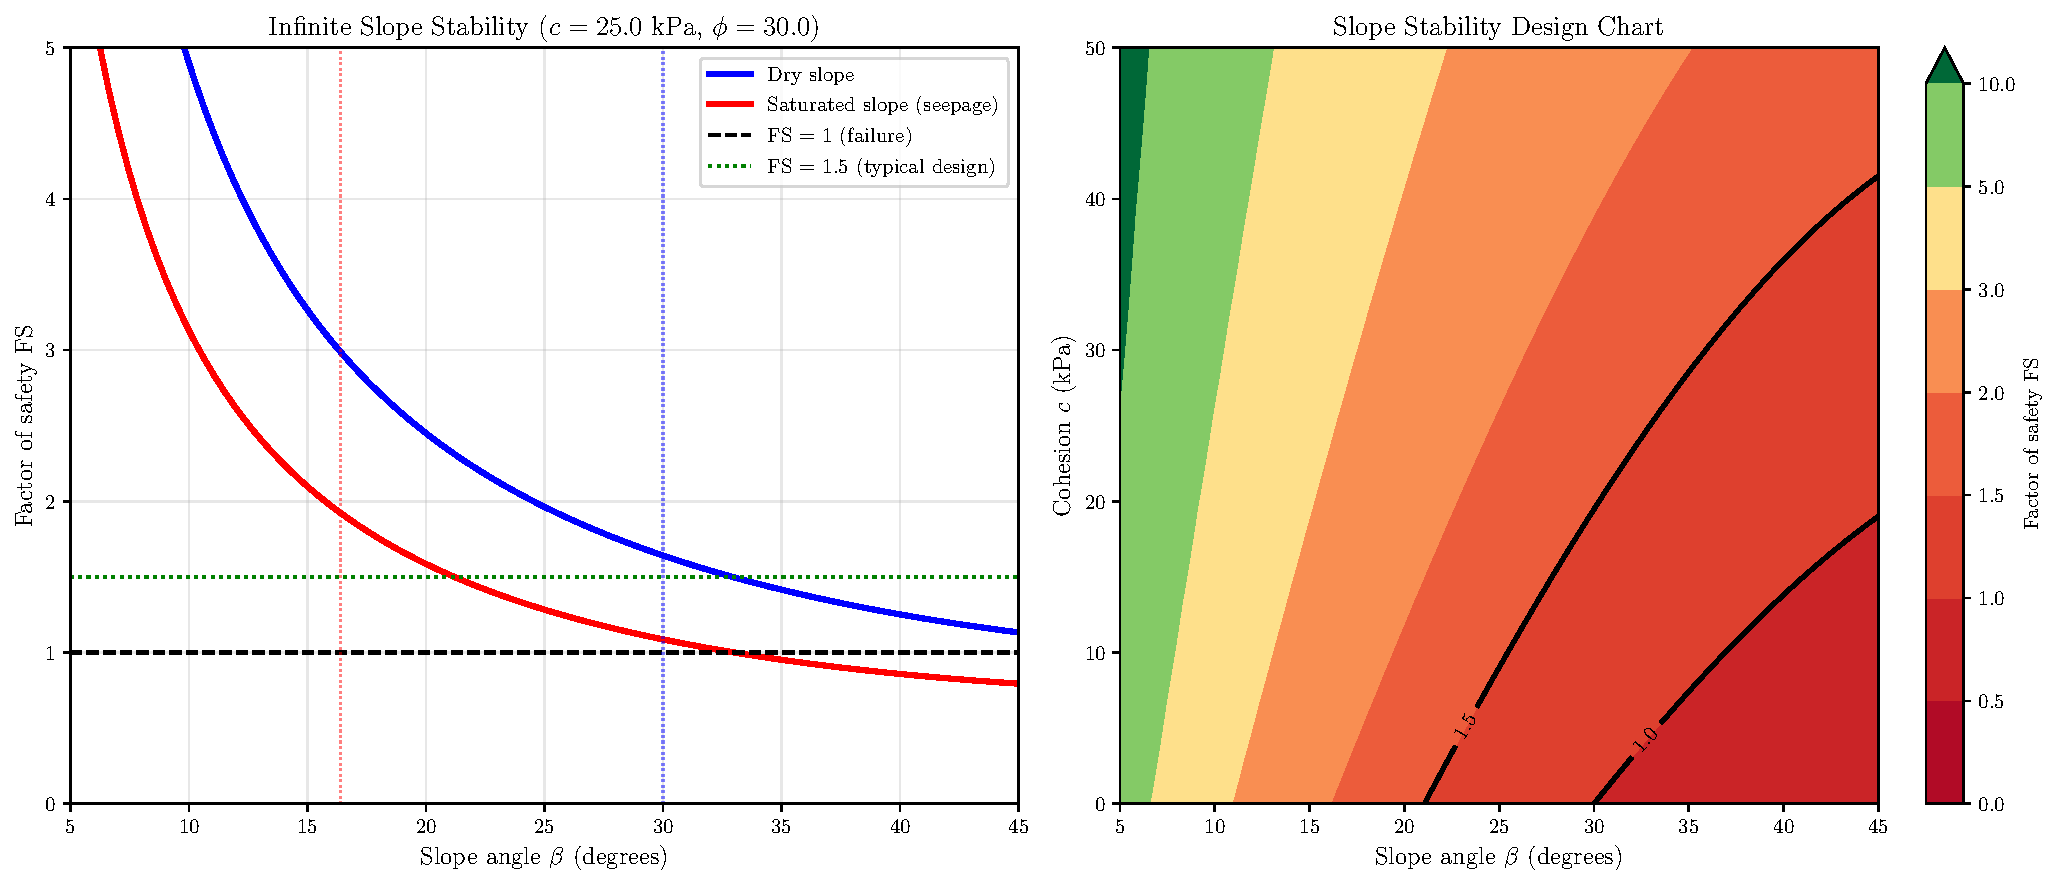
\includegraphics[width=0.98\textwidth]{soil_mechanics_plot5.pdf}
\caption{Left: Factor of safety versus slope angle for infinite slope showing critical importance of groundwater. For a 30° slope, dry conditions give FS = \py{f"{FS_eval_dry[1]:.2f}"} while saturated conditions reduce this to FS = \py{f"{FS_eval_sat[1]:.2f}"}. Critical angle for cohesionless dry soil is \py{f"{beta_crit_dry:.0f}"}° and for saturated soil is \py{f"{beta_crit_sat:.0f}"}°. Right: Design chart showing safe (green) and unstable (red) combinations of slope angle and cohesion. Contours at FS = 1.0 (failure) and 1.5 (typical design minimum) provide rapid assessment. This demonstrates why cohesive soils can sustain steeper slopes and why drainage is critical for slope stability.}
\end{figure}

\section{Compressibility and Settlement}

Soil compressibility governs settlement under foundation loads. The compression index $C_c$ and recompression index $C_r$ define the stress-strain relationship.

\begin{pycode}
# Void ratio vs effective stress (e-log p curve)
sigma_v = np.logspace(1, 3, 100)  # kPa
e0_clay = 1.2
Cc_clay = 0.4
Cr_clay = 0.05
sigma_p = 200  # kPa preconsolidation pressure

# Void ratio calculation
e = np.zeros_like(sigma_v)
for i, sig in enumerate(sigma_v):
    if sig <= sigma_p:
        e[i] = e0_clay - Cr_clay * np.log10(sig / 50)  # reloading
    else:
        e_p = e0_clay - Cr_clay * np.log10(sigma_p / 50)
        e[i] = e_p - Cc_clay * np.log10(sig / sigma_p)  # virgin compression

# Settlement for different OCR values
sigma_v0 = 100  # kPa initial stress
delta_sigma = 150  # kPa load increment
H_layer = 8  # m thickness
OCR_values = [1, 2, 4, 8]  # overconsolidation ratio

settlements = []
for OCR in OCR_values:
    sigma_p_i = OCR * sigma_v0
    if sigma_v0 + delta_sigma <= sigma_p_i:
        # Recompression only
        S = (Cr_clay / (1 + e0_clay)) * H_layer * np.log10((sigma_v0 + delta_sigma) / sigma_v0)
    else:
        # Recompression + virgin compression
        S1 = (Cr_clay / (1 + e0_clay)) * H_layer * np.log10(sigma_p_i / sigma_v0)
        S2 = (Cc_clay / (1 + e0_clay)) * H_layer * np.log10((sigma_v0 + delta_sigma) / sigma_p_i)
        S = S1 + S2
    settlements.append(S * 1000)  # convert to mm

fig, (ax1, ax2) = plt.subplots(1, 2, figsize=(14, 6))

# Left: e-log p curve
ax1.semilogx(sigma_v, e, 'b-', linewidth=2.5)
ax1.axvline(sigma_p, color='r', linestyle='--', linewidth=1.5,
            label=f'Preconsolidation pressure = {sigma_p} kPa')
ax1.set_xlabel('Effective stress $\\sigma_v\'$ (kPa)', fontsize=12)
ax1.set_ylabel('Void ratio $e$', fontsize=12)
ax1.set_title(f'Compressibility Curve ($C_c={Cc_clay}$, $C_r={Cr_clay}$)', fontsize=13)
ax1.legend(loc='upper right', fontsize=10)
ax1.grid(True, alpha=0.3, which='both')
ax1.set_xlim([10, 1000])

# Right: settlement vs OCR
ax2.bar(range(len(OCR_values)), settlements, color='steelblue', edgecolor='black', linewidth=1.5)
ax2.set_xticks(range(len(OCR_values)))
ax2.set_xticklabels([f'OCR={ocr}' for ocr in OCR_values])
ax2.set_ylabel('Settlement (mm)', fontsize=12)
ax2.set_title(f'Settlement vs. Overconsolidation Ratio ($\\Delta\\sigma={delta_sigma}$ kPa)', fontsize=13)
ax2.grid(True, alpha=0.3, axis='y')

for i, s in enumerate(settlements):
    ax2.text(i, s + 5, f'{s:.1f}', ha='center', fontsize=10, fontweight='bold')

plt.tight_layout()
plt.savefig('soil_mechanics_plot6.pdf', dpi=150, bbox_inches='tight')
plt.close()
\end{pycode}

\begin{figure}[H]
\centering
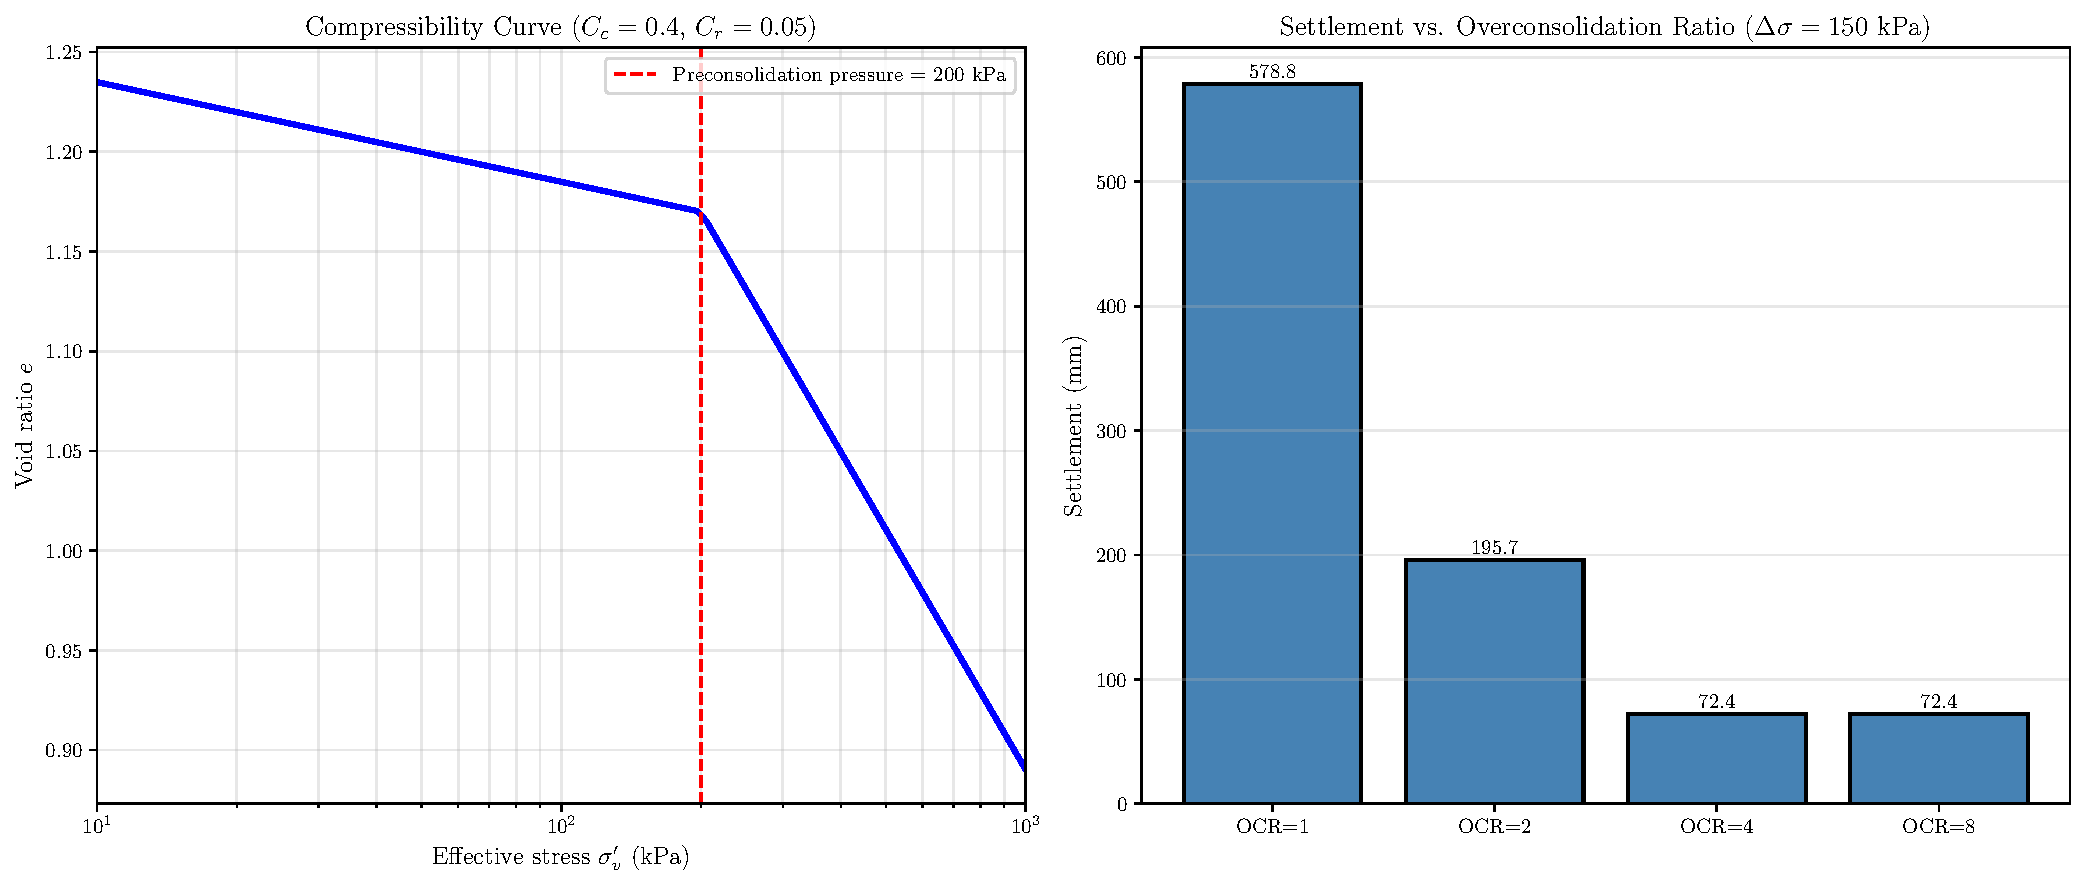
\includegraphics[width=0.98\textwidth]{soil_mechanics_plot6.pdf}
\caption{Left: Void ratio-effective stress relationship showing elastic recompression at low stress (slope $C_r = \py{f"{Cr_clay:.2f}"}$) and virgin compression beyond preconsolidation pressure (slope $C_c = \py{f"{Cc_clay:.2f}"}$). The break in slope at \py{f"{sigma_p}"} kPa indicates stress history. Right: Settlement reduction with increasing overconsolidation ratio (OCR). Normally consolidated clay (OCR=1) settles \py{f"{settlements[0]:.1f}"} mm while heavily overconsolidated clay (OCR=8) settles only \py{f"{settlements[3]:.1f}"} mm under identical loading. This demonstrates why foundation performance depends critically on stress history, motivating preloading and surcharge techniques to reduce post-construction settlement.}
\end{figure}

\section{Results Summary}

The computational analysis yields the following key engineering parameters:

\begin{pycode}
results = [
    ['Ultimate bearing capacity (B=2m)', f'{qu_2m:.0f} kPa'],
    ['Allowable bearing capacity (FS=3)', f'{qa_2m:.0f} kPa'],
    ['Ultimate consolidation settlement', f'{Sc*1000:.1f} mm'],
    ['Time for 50\\% consolidation', f'{t50:.2f} years'],
    ['Time for 90\\% consolidation', f'{t90:.1f} years'],
    ['Bearing capacity factor $N_c$', f'{Nc:.2f}'],
    ['Bearing capacity factor $N_q$', f'{Nq:.2f}'],
    ['Bearing capacity factor $N_\\gamma$', f'{Ngamma:.2f}'],
    ['Slope FS (30°, dry)', f'{FS_eval_dry[1]:.2f}'],
    ['Slope FS (30°, saturated)', f'{FS_eval_sat[1]:.2f}'],
]

print(r'\begin{table}[H]')
print(r'\centering')
print(r'\caption{Summary of Computed Geotechnical Parameters}')
print(r'\begin{tabular}{@{}lc@{}}')
print(r'\toprule')
print(r'Parameter & Value \\')
print(r'\midrule')
for row in results:
    print(f"{row[0]} & {row[1]} \\\\")
print(r'\bottomrule')
print(r'\end{tabular}')
print(r'\end{table}')
\end{pycode}

\section{Conclusions}

This comprehensive analysis demonstrates computational methods for five fundamental aspects of soil mechanics. Effective stress analysis reveals that pore water pressure significantly reduces effective stress below the water table, at 20 m depth reducing effective stress by \py{f"{u_eval[3]/sigma_t_eval[3]*100:.1f}"}\% compared to total stress. Mohr-Coulomb failure analysis shows shear strength is controlled by both cohesion ($c = \py{c}$ kPa) and friction angle ($\phi = \py{phi}°$), with clean sands relying entirely on friction while clays exhibit significant cohesion.

Bearing capacity calculations using Terzaghi's theory yield ultimate capacity $q_u = \py{f"{qu_2m:.0f}"}$ kPa for a 2 m wide footing, giving allowable capacity $q_a = \py{f"{qa_2m:.0f}"}$ kPa with factor of safety FS = \py{f"{FS:.1f}"}. Parametric studies show bearing capacity increases exponentially with friction angle, emphasizing the importance of accurate shear strength characterization.

One-dimensional consolidation analysis predicts ultimate settlement of \py{f"{Sc*1000:.1f}"} mm under 100 kPa surcharge, with 90\% consolidation requiring \py{f"{t90:.1f}"} years. This time-dependent behavior governs staged construction schedules and surcharge design. Slope stability analysis demonstrates the critical importance of groundwater, with saturation reducing factor of safety from \py{f"{FS_eval_dry[1]:.2f}"} to \py{f"{FS_eval_sat[1]:.2f}"} for a 30° slope, explaining the prevalence of slope failures during heavy rainfall.

Compressibility analysis shows that overconsolidation ratio dramatically affects settlement, with OCR = 8 reducing settlement by \py{f"{(1 - settlements[3]/settlements[0])*100:.0f}"}\% compared to normally consolidated soil. This stress history effect is exploited in ground improvement through preloading. The integrated computational framework presented here provides quantitative design tools for foundation engineering, earthwork stability, and settlement prediction, forming the basis for safe and economical geotechnical design.

\bibliographystyle{plain}
\begin{thebibliography}{99}

\bibitem{terzaghi1943}
K. Terzaghi, \textit{Theoretical Soil Mechanics}, John Wiley \& Sons, New York, 1943.

\bibitem{lambe1969}
T. W. Lambe and R. V. Whitman, \textit{Soil Mechanics}, John Wiley \& Sons, New York, 1969.

\bibitem{meyerhof1963}
G. G. Meyerhof, "Some Recent Research on the Bearing Capacity of Foundations," \textit{Canadian Geotechnical Journal}, vol. 1, no. 1, pp. 16--26, 1963.

\bibitem{taylor1948}
D. W. Taylor, \textit{Fundamentals of Soil Mechanics}, John Wiley \& Sons, New York, 1948.

\bibitem{bishop1955}
A. W. Bishop, "The Use of the Slip Circle in the Stability Analysis of Slopes," \textit{Géotechnique}, vol. 5, no. 1, pp. 7--17, 1955.

\bibitem{skempton1957}
A. W. Skempton, "Discussion: The Planning and Design of New Hong Kong Airport," \textit{Proceedings of the Institution of Civil Engineers}, vol. 7, pp. 305--307, 1957.

\bibitem{casagrande1936}
A. Casagrande, "The Determination of the Pre-consolidation Load and Its Practical Significance," \textit{Proceedings of the 1st International Conference on Soil Mechanics and Foundation Engineering}, vol. 3, pp. 60--64, 1936.

\bibitem{bjerrum1967}
L. Bjerrum, "Engineering Geology of Norwegian Normally-Consolidated Marine Clays," \textit{Géotechnique}, vol. 17, no. 2, pp. 81--118, 1967.

\bibitem{das2010}
B. M. Das, \textit{Principles of Geotechnical Engineering}, 7th ed., Cengage Learning, 2010.

\bibitem{vesic1973}
A. S. Vesic, "Analysis of Ultimate Loads of Shallow Foundations," \textit{Journal of the Soil Mechanics and Foundations Division}, ASCE, vol. 99, no. SM1, pp. 45--73, 1973.

\bibitem{janbu1973}
N. Janbu, "Slope Stability Computations," in \textit{Embankment Dam Engineering: Casagrande Volume}, R. C. Hirschfeld and S. J. Poulos, Eds., John Wiley \& Sons, 1973, pp. 47--86.

\bibitem{holtz1981}
R. D. Holtz and W. D. Kovacs, \textit{An Introduction to Geotechnical Engineering}, Prentice-Hall, 1981.

\bibitem{craig2004}
R. F. Craig, \textit{Craig's Soil Mechanics}, 7th ed., Spon Press, 2004.

\bibitem{duncan1970}
J. M. Duncan and C.-Y. Chang, "Nonlinear Analysis of Stress and Strain in Soils," \textit{Journal of the Soil Mechanics and Foundations Division}, ASCE, vol. 96, no. SM5, pp. 1629--1653, 1970.

\bibitem{schofield1968}
A. N. Schofield and C. P. Wroth, \textit{Critical State Soil Mechanics}, McGraw-Hill, London, 1968.

\bibitem{roscoe1968}
K. H. Roscoe and J. B. Burland, "On the Generalized Stress-Strain Behaviour of 'Wet' Clay," in \textit{Engineering Plasticity}, J. Heyman and F. A. Leckie, Eds., Cambridge University Press, 1968, pp. 535--609.

\bibitem{bowles1996}
J. E. Bowles, \textit{Foundation Analysis and Design}, 5th ed., McGraw-Hill, 1996.

\bibitem{peck1974}
R. B. Peck, W. E. Hanson, and T. H. Thornburn, \textit{Foundation Engineering}, 2nd ed., John Wiley \& Sons, 1974.

\bibitem{morgenstern1965}
N. R. Morgenstern and V. E. Price, "The Analysis of the Stability of General Slip Surfaces," \textit{Géotechnique}, vol. 15, no. 1, pp. 79--93, 1965.

\bibitem{wroth1984}
C. P. Wroth, "The Interpretation of In Situ Soil Tests," \textit{Géotechnique}, vol. 34, no. 4, pp. 449--489, 1984.

\end{thebibliography}

\end{document}
